

\tikzset{every picture/.style={line width=0.75pt}} %set default line width to 0.75pt        

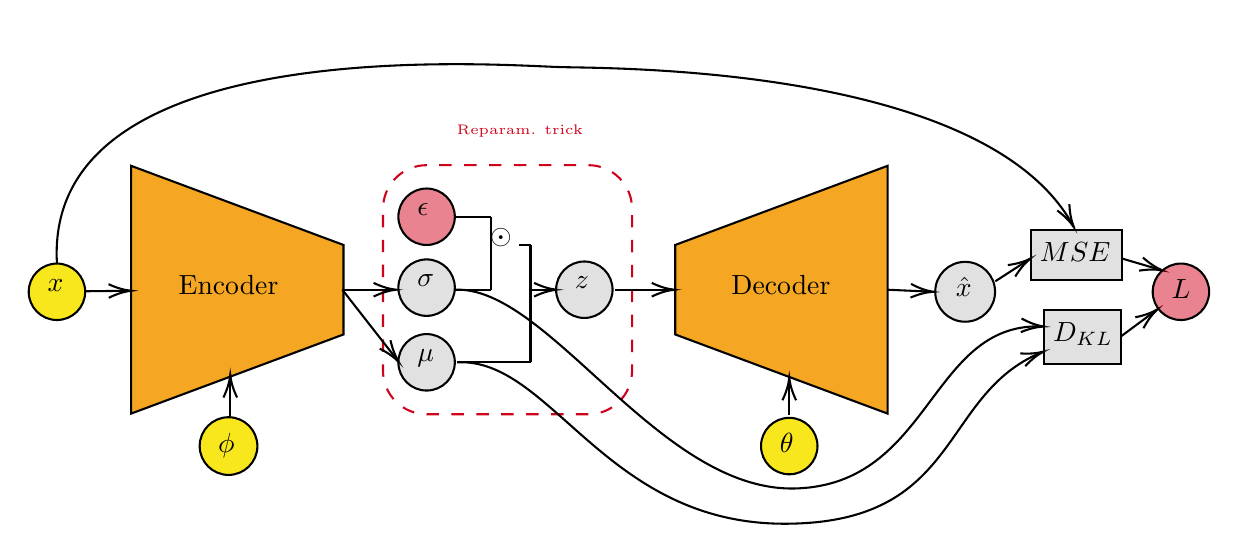
\begin{tikzpicture}[x=0.75pt,y=0.75pt,yscale=-1,xscale=1]
%uncomment if require: \path (0,300); %set diagram left start at 0, and has height of 300

%Shape: Trapezoid [id:dp4603381933629067] 
\draw  [fill={rgb, 255:red, 245; green, 166; blue, 35 }  ,fill opacity=1 ] (93.26,100.32) -- (195.56,138.44) -- (195.56,181.56) -- (93.26,219.68) -- cycle ;
%Flowchart: Alternative Process [id:dp9485975912798454] 
\draw  [color={rgb, 255:red, 208; green, 2; blue, 27 }  ,draw opacity=1 ][dash pattern={on 4.5pt off 4.5pt}] (313.6,100) .. controls (325.2,100) and (334.6,109.4) .. (334.6,121) -- (334.6,199) .. controls (334.6,210.6) and (325.2,220) .. (313.6,220) -- (235.6,220) .. controls (224,220) and (214.6,210.6) .. (214.6,199) -- (214.6,121) .. controls (214.6,109.4) and (224,100) .. (235.6,100) -- cycle ;
%Shape: Trapezoid [id:dp05976858710421107] 
\draw  [fill={rgb, 255:red, 245; green, 166; blue, 35 }  ,fill opacity=1 ] (457.69,219.68) -- (355.39,181.56) -- (355.39,138.44) -- (457.69,100.32) -- cycle ;
%Straight Lines [id:da8886776302625958] 
\draw    (71,160.75) -- (91.33,160.52) ;
\draw [shift={(93.33,160.5)}, rotate = 179.36] [color={rgb, 255:red, 0; green, 0; blue, 0 }  ][line width=0.75]    (10.93,-3.29) .. controls (6.95,-1.4) and (3.31,-0.3) .. (0,0) .. controls (3.31,0.3) and (6.95,1.4) .. (10.93,3.29)   ;
%Straight Lines [id:da08810248930582953] 
\draw    (141,221.67) -- (141,203) ;
\draw [shift={(141,201)}, rotate = 90] [color={rgb, 255:red, 0; green, 0; blue, 0 }  ][line width=0.75]    (10.93,-3.29) .. controls (6.95,-1.4) and (3.31,-0.3) .. (0,0) .. controls (3.31,0.3) and (6.95,1.4) .. (10.93,3.29)   ;
%Straight Lines [id:da09541704278112628] 
\draw    (457.67,160) -- (477.8,160.91) ;
\draw [shift={(479.8,161)}, rotate = 182.59] [color={rgb, 255:red, 0; green, 0; blue, 0 }  ][line width=0.75]    (10.93,-3.29) .. controls (6.95,-1.4) and (3.31,-0.3) .. (0,0) .. controls (3.31,0.3) and (6.95,1.4) .. (10.93,3.29)   ;
%Straight Lines [id:da7627795640935963] 
\draw    (410.33,220.33) -- (410.33,204.33) ;
\draw [shift={(410.33,202.33)}, rotate = 90] [color={rgb, 255:red, 0; green, 0; blue, 0 }  ][line width=0.75]    (10.93,-3.29) .. controls (6.95,-1.4) and (3.31,-0.3) .. (0,0) .. controls (3.31,0.3) and (6.95,1.4) .. (10.93,3.29)   ;
%Straight Lines [id:da9671113396067061] 
\draw    (249.67,124.84) -- (266.6,124.84) ;
%Straight Lines [id:da49282311320645533] 
\draw    (249,160) -- (266.6,160) ;
%Straight Lines [id:da5997141555105364] 
\draw    (266.6,124.84) -- (266.6,160) ;
%Straight Lines [id:da0115478599512705] 
\draw    (285.67,194.98) -- (250.33,194.98) ;
%Straight Lines [id:da4324256163961162] 
\draw    (285.67,138.44) -- (285.67,194.98) ;
%Straight Lines [id:da9272156374696123] 
\draw    (280.33,138.44) -- (285.67,138.44) ;
%Straight Lines [id:da4926352715342106] 
\draw    (285.67,160) -- (296.33,160) ;
\draw [shift={(298.33,160)}, rotate = 180] [color={rgb, 255:red, 0; green, 0; blue, 0 }  ][line width=0.75]    (10.93,-3.29) .. controls (6.95,-1.4) and (3.31,-0.3) .. (0,0) .. controls (3.31,0.3) and (6.95,1.4) .. (10.93,3.29)   ;
%Straight Lines [id:da04537908983318728] 
\draw    (326.33,160) -- (353,160) ;
\draw [shift={(355,160)}, rotate = 180] [color={rgb, 255:red, 0; green, 0; blue, 0 }  ][line width=0.75]    (10.93,-3.29) .. controls (6.95,-1.4) and (3.31,-0.3) .. (0,0) .. controls (3.31,0.3) and (6.95,1.4) .. (10.93,3.29)   ;
%Straight Lines [id:da7906963000638052] 
\draw    (195,160) -- (219,160) ;
\draw [shift={(221,160)}, rotate = 180] [color={rgb, 255:red, 0; green, 0; blue, 0 }  ][line width=0.75]    (10.93,-3.29) .. controls (6.95,-1.4) and (3.31,-0.3) .. (0,0) .. controls (3.31,0.3) and (6.95,1.4) .. (10.93,3.29)   ;
%Straight Lines [id:da8571872389936455] 
\draw    (195,160) -- (221.1,193.4) ;
\draw [shift={(222.33,194.98)}, rotate = 232] [color={rgb, 255:red, 0; green, 0; blue, 0 }  ][line width=0.75]    (10.93,-3.29) .. controls (6.95,-1.4) and (3.31,-0.3) .. (0,0) .. controls (3.31,0.3) and (6.95,1.4) .. (10.93,3.29)   ;
%Curve Lines [id:da13814007069926393] 
\draw    (249,160) .. controls (294.33,157.67) and (347.5,257.75) .. (413.5,255.75) .. controls (478.84,253.77) and (478.02,176.32) .. (531.37,177.68) ;
\draw [shift={(533,177.75)}, rotate = 183.12] [color={rgb, 255:red, 0; green, 0; blue, 0 }  ][line width=0.75]    (10.93,-3.29) .. controls (6.95,-1.4) and (3.31,-0.3) .. (0,0) .. controls (3.31,0.3) and (6.95,1.4) .. (10.93,3.29)   ;
%Curve Lines [id:da05365168320135172] 
\draw    (250.33,194.98) .. controls (295.67,192.65) and (321.33,272.75) .. (408,272.75) .. controls (493.8,272.75) and (482.24,211) .. (531.49,190.36) ;
\draw [shift={(533,189.75)}, rotate = 158.59] [color={rgb, 255:red, 0; green, 0; blue, 0 }  ][line width=0.75]    (10.93,-3.29) .. controls (6.95,-1.4) and (3.31,-0.3) .. (0,0) .. controls (3.31,0.3) and (6.95,1.4) .. (10.93,3.29)   ;
%Curve Lines [id:da8232139075562327] 
\draw    (57.5,147.25) .. controls (51,34.25) and (272.5,52.08) .. (300.5,52.75) .. controls (328.36,53.41) and (504.72,52.76) .. (546.87,128.8) ;
\draw [shift={(547.5,129.95)}, rotate = 242.03] [color={rgb, 255:red, 0; green, 0; blue, 0 }  ][line width=0.75]    (10.93,-3.29) .. controls (6.95,-1.4) and (3.31,-0.3) .. (0,0) .. controls (3.31,0.3) and (6.95,1.4) .. (10.93,3.29)   ;
%Straight Lines [id:da7274853980914816] 
\draw    (509.6,155.95) -- (524.92,146.04) ;
\draw [shift={(526.6,144.95)}, rotate = 147.09] [color={rgb, 255:red, 0; green, 0; blue, 0 }  ][line width=0.75]    (10.93,-3.29) .. controls (6.95,-1.4) and (3.31,-0.3) .. (0,0) .. controls (3.31,0.3) and (6.95,1.4) .. (10.93,3.29)   ;
%Straight Lines [id:da4317146239738564] 
\draw    (570.97,145.07) -- (588.38,150.19) ;
\draw [shift={(590.3,150.75)}, rotate = 196.38] [color={rgb, 255:red, 0; green, 0; blue, 0 }  ][line width=0.75]    (10.93,-3.29) .. controls (6.95,-1.4) and (3.31,-0.3) .. (0,0) .. controls (3.31,0.3) and (6.95,1.4) .. (10.93,3.29)   ;
%Straight Lines [id:da8631782029369521] 
\draw    (570,182.6) -- (586.19,170.59) ;
\draw [shift={(587.8,169.4)}, rotate = 143.44] [color={rgb, 255:red, 0; green, 0; blue, 0 }  ][line width=0.75]    (10.93,-3.29) .. controls (6.95,-1.4) and (3.31,-0.3) .. (0,0) .. controls (3.31,0.3) and (6.95,1.4) .. (10.93,3.29)   ;

% Text Node
\draw  [fill={rgb, 255:red, 248; green, 231; blue, 28 }  ,fill opacity=1 ]  (57.5, 161) circle [x radius= 13.6, y radius= 13.6]   ;
\draw (51.5,153.4) node [anchor=north west][inner sep=0.75pt]    {$x$};
% Text Node
\draw (114.67,151.5) node [anchor=north west][inner sep=0.75pt]   [align=left] {Encoder};
% Text Node
\draw (381,151.5) node [anchor=north west][inner sep=0.75pt]   [align=left] {Decoder};
% Text Node
\draw  [fill={rgb, 255:red, 155; green, 155; blue, 155 }  ,fill opacity=0.3 ]  (495.07, 161) circle [x radius= 14.42, y radius= 14.42]   ;
\draw (489.07,152.4) node [anchor=north west][inner sep=0.75pt]    {$\hat{x}$};
% Text Node
\draw  [fill={rgb, 255:red, 248; green, 231; blue, 28 }  ,fill opacity=1 ]  (140.17, 235.33) circle [x radius= 13.9, y radius= 13.9]   ;
\draw (133.67,227.73) node [anchor=north west][inner sep=0.75pt]    {$\phi $};
% Text Node
\draw  [fill={rgb, 255:red, 208; green, 2; blue, 27 }  ,fill opacity=0.49 ]  (235.6, 124.84) circle [x radius= 13.6, y radius= 13.6]   ;
\draw (229.6,117.24) node [anchor=north west][inner sep=0.75pt]    {$\epsilon $};
% Text Node
\draw  [fill={rgb, 255:red, 248; green, 231; blue, 28 }  ,fill opacity=1 ]  (410.33, 235.33) circle [x radius= 13.6, y radius= 13.6]   ;
\draw (404.33,227.73) node [anchor=north west][inner sep=0.75pt]    {$\theta $};
% Text Node
\draw  [fill={rgb, 255:red, 155; green, 155; blue, 155 }  ,fill opacity=0.3 ]  (235.6, 159) circle [x radius= 13.6, y radius= 13.6]   ;
\draw (229.6,151.4) node [anchor=north west][inner sep=0.75pt]    {$\sigma $};
% Text Node
\draw  [fill={rgb, 255:red, 155; green, 155; blue, 155 }  ,fill opacity=0.3 ]  (235.6, 194.98) circle [x radius= 13.6, y radius= 13.6]   ;
\draw (229.6,187.38) node [anchor=north west][inner sep=0.75pt]    {$\mu $};
% Text Node
\draw  [fill={rgb, 255:red, 155; green, 155; blue, 155 }  ,fill opacity=0.3 ]  (311.6, 160) circle [x radius= 13.6, y radius= 13.6]   ;
\draw (305.6,152.4) node [anchor=north west][inner sep=0.75pt]    {$z$};
% Text Node
\draw (264.67,128.84) node [anchor=north west][inner sep=0.75pt]    {$\odot $};
% Text Node
\draw  [fill={rgb, 255:red, 155; green, 155; blue, 155 }  ,fill opacity=0.3 ]  (526.6,131.34) -- (570.6,131.34) -- (570.6,155.34) -- (526.6,155.34) -- cycle  ;
\draw (529.6,135.74) node [anchor=north west][inner sep=0.75pt]    {$MSE$};
% Text Node
\draw  [fill={rgb, 255:red, 155; green, 155; blue, 155 }  ,fill opacity=0.3 ]  (533,169.96) -- (570,169.96) -- (570,195.96) -- (533,195.96) -- cycle  ;
\draw (536,174.36) node [anchor=north west][inner sep=0.75pt]    {$D_{KL}$};
% Text Node
\draw (248.67,79) node [anchor=north west][inner sep=0.75pt]  [color={rgb, 255:red, 208; green, 2; blue, 27 }  ,opacity=1 ] [align=left] {{\tiny Reparam. trick}};
% Text Node
\draw  [fill={rgb, 255:red, 208; green, 2; blue, 27 }  ,fill opacity=0.49 ]  (599.03, 161) circle [x radius= 13.6, y radius= 13.6]   ;
\draw (593.03,153.4) node [anchor=north west][inner sep=0.75pt]    {$L$};


\end{tikzpicture}
